\documentclass{beamer}
%
% Choose how your presentation looks.
%
% For more themes, color themes and font themes, see:
% http://deic.uab.es/~iblanes/beamer_gallery/index_by_theme.html
%
\mode<presentation>
{
  \usetheme{Boadilla}      % or try Darmstadt, Madrid, Warsaw, ...
  \usecolortheme{beaver} % or try albatross, beaver, crane, ...
  \usefonttheme{default}  % or try serif, structurebold, ...
  \setbeamertemplate{navigation symbols}{}
  \setbeamertemplate{caption}[numbered]
  
} 

\usepackage{xcolor,colortbl}
\usepackage[english]{babel}
\usepackage[utf8x]{inputenc}
\usepackage{courier}
\usepackage{dsfont}
\usepackage{verbatim} 
\usepackage{enumerate}
\usepackage{tikz}
\usepackage{multirow}
\usepackage{bbm}
\usepackage{amsmath}
\usepackage{venndiagram}
\usepackage{epigraph} 
%\usepackage{xcolor}

%\usepackage{enumitem}

\usepackage{hyperref}
\hypersetup{
    colorlinks=true,
    linkcolor=blue,
    filecolor=magenta,      
    urlcolor=cyan,
}

% R stuff!
\usepackage{listings}
\definecolor{codegreen}{rgb}{0,0.6,0}
\definecolor{codegray}{rgb}{0.5,0.5,0.5}
\definecolor{codepurple}{rgb}{0.58,0,0.82}
\definecolor{backcolour}{rgb}{0.95,0.95,0.92}

\lstdefinestyle{mystyle}{
    backgroundcolor=\color{backcolour},    
    commentstyle=\color{codegreen},
    keywordstyle=\color{black},
    numberstyle=\tiny\color{codegray},
    stringstyle=\color{codepurple},
    basicstyle=\ttfamily\footnotesize,
    breakatwhitespace=false,         
    breaklines=true,                 
    captionpos=b,                    
    keepspaces=true,                 
    numbers=left,                    
    numbersep=5pt,                  
    showspaces=false,                
    showstringspaces=false,
    showtabs=false,                  
    tabsize=2
}

\lstset{style=mystyle}



%% Size options for nested itemized lists
\usepackage{relsize}
\setbeamerfont{itemize/enumerate body}{parent=normal text}
\setbeamerfont{itemize/enumerate subbody}{parent=normal text,size=\relsize{-1}}
%\setbeamerfont{itemize/enumerate subsubbody}{parent=normal text,size=\relsize{-1}}




\setbeamertemplate{enumerate items}[default]
\setbeamertemplate{itemize item}[triangle]

%\setitemize{label=\usebeamerfont*{itemize item}%
%  \usebeamercolor[fg]{itemize item}
%  \usebeamertemplate{itemize item}}


\usetikzlibrary{shapes,decorations,arrows,calc,arrows.meta,fit,positioning}
\tikzset{
    -Latex,auto,node distance =1 cm and 1 cm,semithick,
    state/.style ={ellipse, draw, minimum width = 0.7 cm},
    point/.style = {circle, draw, inner sep=0.04cm,fill,node contents={}},
    bidirected/.style={Latex-Latex,dashed},
    el/.style = {inner sep=2pt, align=left, sloped}
}

\newcommand{\Mypm}{\mathbin{\tikz [x=1.4ex,y=1.4ex,line width=.1ex] \draw (0.0,0) -- (1.0,0) (0.5,0.08) -- (0.5,0.92) (0.0,0.5) -- (1.0,0.5);}}%



%% For block quote
\usepackage{etoolbox}
\AtBeginEnvironment{quote}{\par\singlespacing\small}


\title[STA 209]{ANOVA Part 2}
\subtitle{}
%\author{}
\author{Grinnell College}
\date{December 4, 2024}

\graphicspath{{img/}}

\begin{document}

\begin{frame}
  \titlepage
\end{frame}

\begin{frame}{Review}

\begin{itemize}
\item What were we doing with ANOVA?
\item What was the F-statistic representing?
\item Maybe let's have fewer equations today

\end{itemize}


\end{frame}


\begin{frame}{Speed of all dogs}
Jitter Plot (better than boxplot for this example)
\begin{center}
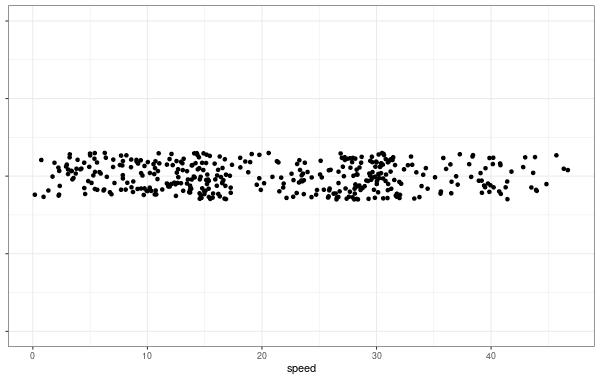
\includegraphics[scale=0.45]{all_dog_speed.png}
\end{center}
\end{frame}


\begin{frame}{Speed of all dogs}
\small
\begin{center}
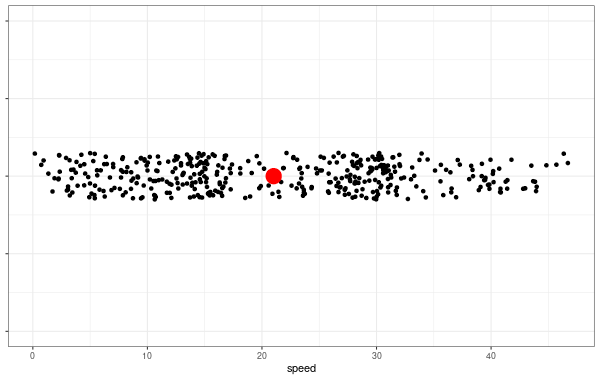
\includegraphics[scale=0.45]{all_dog_speed_mean.png}
\end{center}
% latex table generated in R 4.3.3 by xtable 1.8-4 package
% Fri Apr 26 08:54:59 2024
\begin{table}[ht]
\centering
\begin{tabular}{lrrrrr}
  \hline
 & Df & Sum Sq & Mean Sq & F value & Pr($>$F) \\ 
  \hline
Residuals   & 399 & 52398 & 131.32 &  &  \\ 
   \hline
\end{tabular}
\end{table}
\end{frame}



\begin{frame}{Speed of Size dogs}
\begin{center}
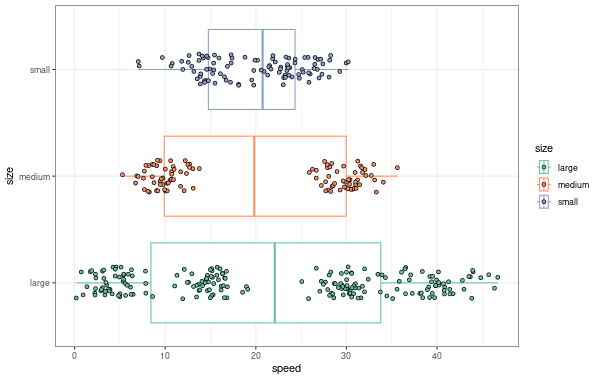
\includegraphics[scale=0.45]{size_dog_speed.png}
\end{center}
\end{frame}


\begin{frame}{Speed of Size dogs}
\small
\begin{center}
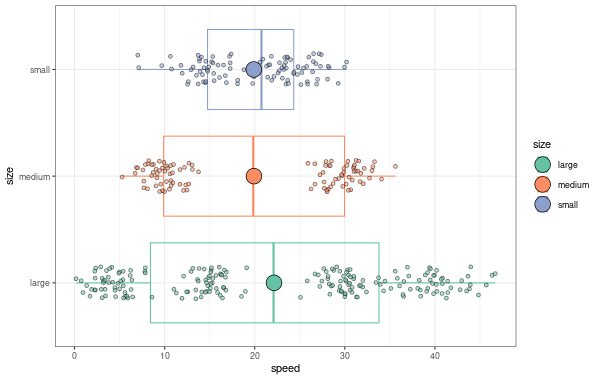
\includegraphics[scale=0.45]{size_dog_speed_mean.png}
\end{center}
\begin{table}[ht]
\centering
\begin{tabular}{lrrrrr}
  \hline
 & Df & Sum Sq & Mean Sq & F value & Pr($>$F) \\ 
  \hline
size        & 2 & 498 & 248.96 & 1.90 & 0.1503 \\ 
  Residuals   & 397 & 51900 & 130.73 &  &  \\ 
   \hline
\end{tabular}
\end{table}
\end{frame}



\begin{frame}{Speed of Color dogs}
\begin{center}
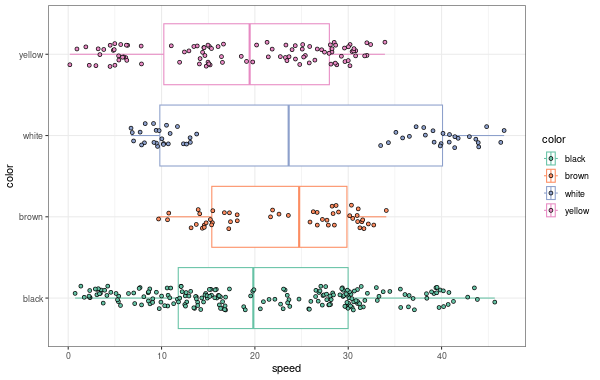
\includegraphics[scale=0.45]{color_dog_speed.png}
\end{center}
\end{frame}


\begin{frame}{Speed of Color dogs}
\small
\begin{center}
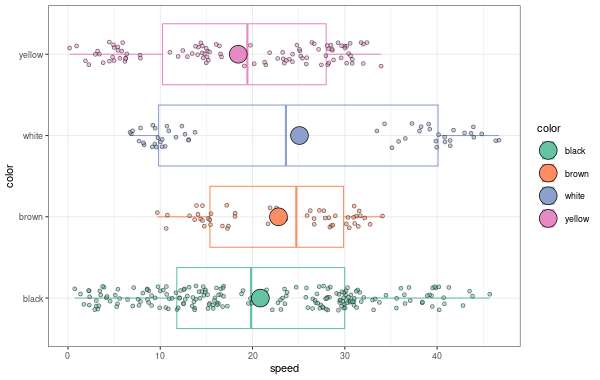
\includegraphics[scale=0.45]{color_dog_speed_mean.png}
\end{center}
% latex table generated in R 4.3.3 by xtable 1.8-4 package
% Fri Apr 26 09:00:35 2024
\begin{table}[ht]
\centering
\begin{tabular}{lrrrrr}
  \hline
 & Df & Sum Sq & Mean Sq & F value & Pr($>$F) \\ 
  \hline
color       & 3 & 1652 & 550.55 & 4.30 & 0.0053 \\ 
  Residuals   & 396 & 50746 & 128.15 &  &  \\ 
   \hline
\end{tabular}
\end{table}
\end{frame}



\begin{frame}{Speed of Breed dogs}
\begin{center}
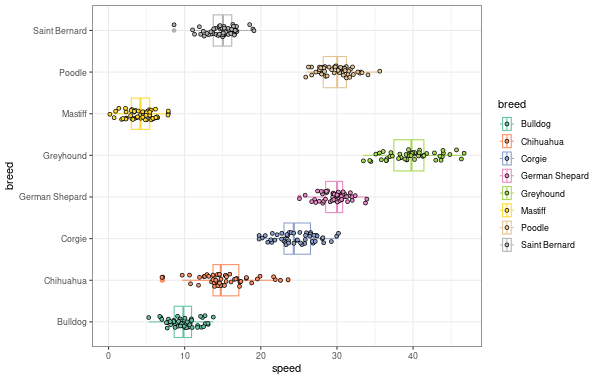
\includegraphics[scale=0.45]{breed_dog_speed.png}
\end{center}
\end{frame}


\begin{frame}{Speed of Breed dogs}
\small
\begin{center}
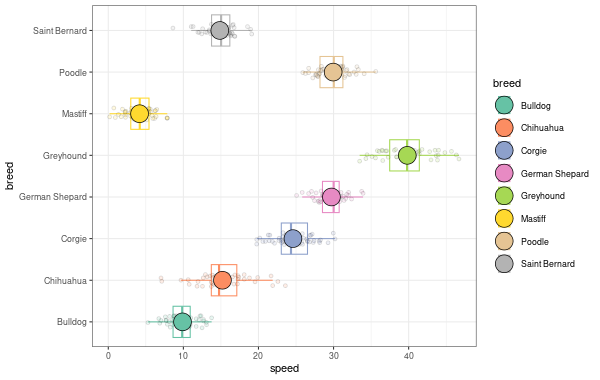
\includegraphics[scale=0.45]{breed_dog_speed_mean.png}
\end{center}
% latex table generated in R 4.3.3 by xtable 1.8-4 package
% Fri Apr 26 09:02:23 2024
\begin{table}[ht]
\centering
\begin{tabular}{lrrrrr}
  \hline
 & Df & Sum Sq & Mean Sq & F value & Pr($>$F) \\ 
  \hline
breed       & 7 & 50066 & 7152.25 & 1202.16 & 0.0000 \\ 
  Residuals   & 392 & 2332 & 5.95 &  &  \\ 
   \hline
\end{tabular}
\end{table}
\end{frame}


\begin{frame}{To $t$ or Not to $t$}

Recall that for ANOVA we are testing the null hypothesis that \textit{all} of our means our equal
\begin{align*}
H_0: \mu_A = \mu_B = \mu_C
\end{align*}
\vspace{2mm}

Why not instead just stick with our t-test, doing
\begin{align*}
H_0: \mu_A = \mu_B, \ \mu_A = \mu_C, \text{ and } \mu_B = \mu_C
\end{align*}

\end{frame}


\begin{frame}{Multiple tests}
15 groups, all generated with the same mean value:
\begin{itemize}
    \item F-test (ANOVA) should not tell us there is a difference
\end{itemize}
\begin{center}
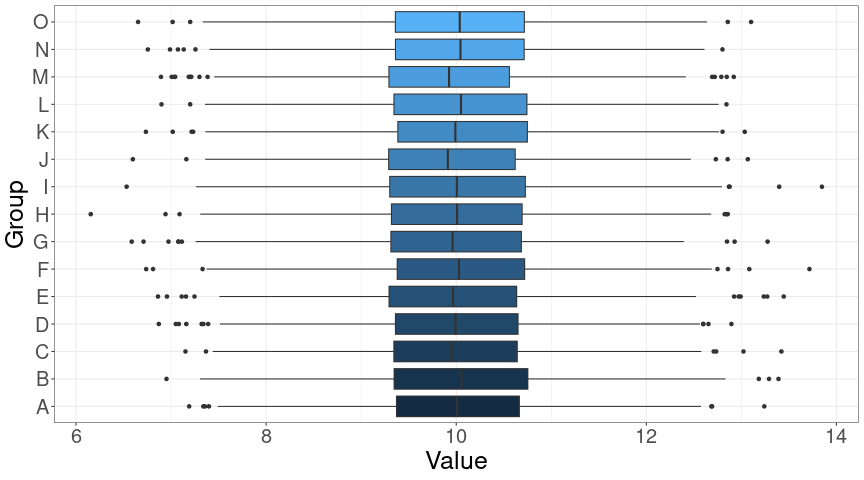
\includegraphics[scale=0.38]{allgps.png}
\end{center}
\end{frame}

\begin{frame}{Multiple tests}
\small
\begin{center}
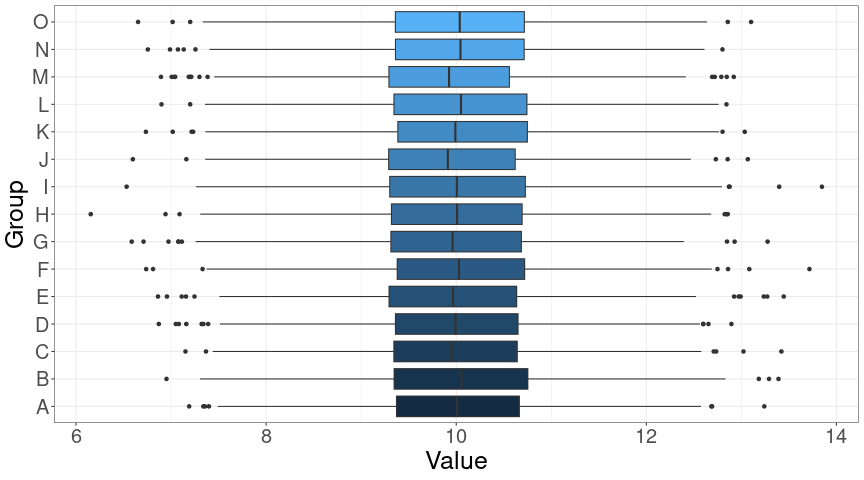
\includegraphics[scale=0.35]{allgps.png}
\end{center}
% latex table generated in R 4.3.3 by xtable 1.8-4 package
% Fri Apr 26 09:38:19 2024
\begin{table}[ht]
\centering
\begin{tabular}{lrrrrr}
  \hline
 & Df & Sum Sq & Mean Sq & F value & Pr($>$F) \\ 
  \hline
Group       & 14 & 15.40 & 1.10 & 1.10 & 0.3504 \\ 
  Residuals   & 14985 & 14964.85 & 1.00 &  &  \\ 
   \hline
\end{tabular}
\end{table}

\end{frame}

\begin{frame}{Multiple tests}
\begin{itemize}
\item 105 pair-wise tests
\item 6 with $p$-value $< 0.05$
\end{itemize}
\begin{center}
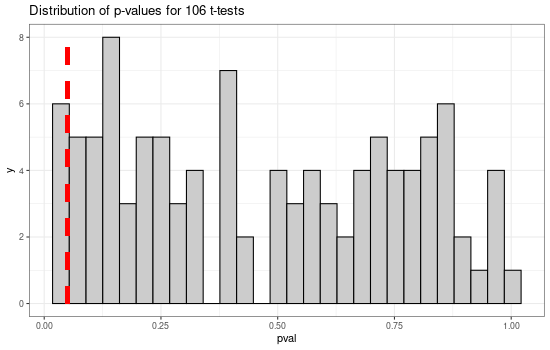
\includegraphics[scale=0.5]{pval_hist.png}
\end{center}
\end{frame}

\begin{frame}{Post-hoc Tests}
ANOVA only tells us \textit{that} a difference exists, not where it is or to what degree \vspace{8mm}

If our ANOVA test is such that we reject the null hypothesis, we can use \textit{post-hoc} testing via the \textbf{Tukey Range Test} or the \textbf{Tukey Honest Significant Difference Test} to identify any statistically significant pair-wise differences
\end{frame}

\begin{frame}
\begin{center}
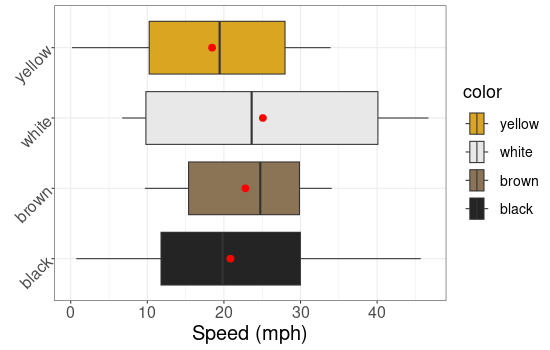
\includegraphics[scale=0.5]{dog_color_2.png}
\end{center}
% latex table generated in R 4.3.3 by xtable 1.8-4 package
% Fri Apr 26 09:59:16 2024
\begin{table}[ht]
\centering
\begin{tabular}{lrrrrr}
  \hline
 & Df & Sum Sq & Mean Sq & F value & Pr($>$F) \\ 
  \hline
color       & 3 & 1651.64 & 550.55 & 4.30 & 0.0053 \\ 
  Residuals   & 396 & 50746.34 & 128.15 &  &  \\ 
   \hline
\end{tabular}
\end{table}
\end{frame}

\begin{frame}[fragile]

\begin{lstlisting}[language=R]
> aov(speed ~ color, dogs) %>% TukeyHSD() 
  Tukey multiple comparisons of means
    95% family-wise confidence level

Fit: aov(formula = speed ~ color, data = dogs)

$color
                diff       lwr      upr   p adj
brown-black   1.9612  -2.65664  6.57906 0.69237
white-black   4.2360  -0.38182  8.85388 0.08529
yellow-black -2.3968  -5.97373  1.18021 0.31012
white-brown   2.2748  -3.56635  8.11599 0.74672
yellow-brown -4.3580  -9.41657  0.70063 0.11889
yellow-white -6.6328 -11.69139 -1.57418 0.00437
\end{lstlisting}

\end{frame}

\begin{frame}[fragile]

\begin{lstlisting}[language=R]
> aov(speed ~ color, dogs) %>% TukeyHSD() %>% plot()
\end{lstlisting}
\begin{center}
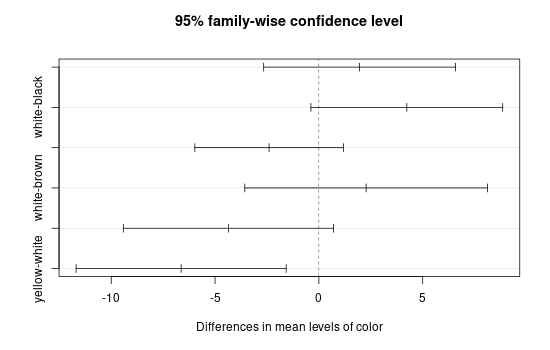
\includegraphics[scale=0.5]{tukeyhsd.png}
\end{center}
\end{frame}

\begin{frame}{Review}

\begin{itemize}
\item ANOVA allows us to test equality of many means
\begin{itemize}
\item By comparing ratio of between-group and within-group variance
\end{itemize}
\item alleviates problem of multiple testing
\item \textit{Post-hoc} testing can be done to determine which groups are different
\item Tukey Honest Statistical Difference (TukeyHSD)
\end{itemize}

\end{frame}


%\begin{frame}
%\begin{columns}
%
%  \begin{column}{0.45\textwidth}
%%
%  \end{column}
%  \begin{column}{0.45\textwidth}
%%
%  \end{column}
%
%\end{columns}
%\end{frame}


\end{document}
